
\documentclass{article}
\usepackage[utf8]{inputenc}
\usepackage[margin=1in,left=1.5in,includefoot]{geometry}
\usepackage{booktabs}
\usepackage{amsmath}
\usepackage{amsfonts}
\usepackage{booktabs}
\usepackage[spanish]{babel}
\usepackage{graphicx}
\usepackage{caption}
\usepackage[most]{tcolorbox}
\usepackage{lmodern}
\usepackage{listings}
\usepackage{epigraph}
\usepackage{hyperref}
% Header & Footer Stuff

\addto\captionsspanish{%
  \renewcommand{\figurename}{Figura}%
  \renewcommand{\tablename}{Táboa}%
}

\setlength{\epigraphwidth}{0.7\textwidth}

\usepackage{fancyhdr}
\pagestyle{fancy}
\lhead{Modelos Avanzados de Aprendizaxe Automático II}
\rhead{614G030302425}
% \fancyfoot{}
% \lfoot{Pablo Chantada Saborido \& José Romero Conde}
% \fancyfoot[R]{}

% The Main Document
\begin{document}
\begin{center}
    \LARGE\bfseries PRÁCTICA III \\
    \large \emph{Aprendizaxe por reforzo} \\
    \small Pablo Chantada Saborido \& José Romero Conde
    \line(1,0){430}
\end{center}

\vspace{200}
\begin{figure}[h]
    \centering
    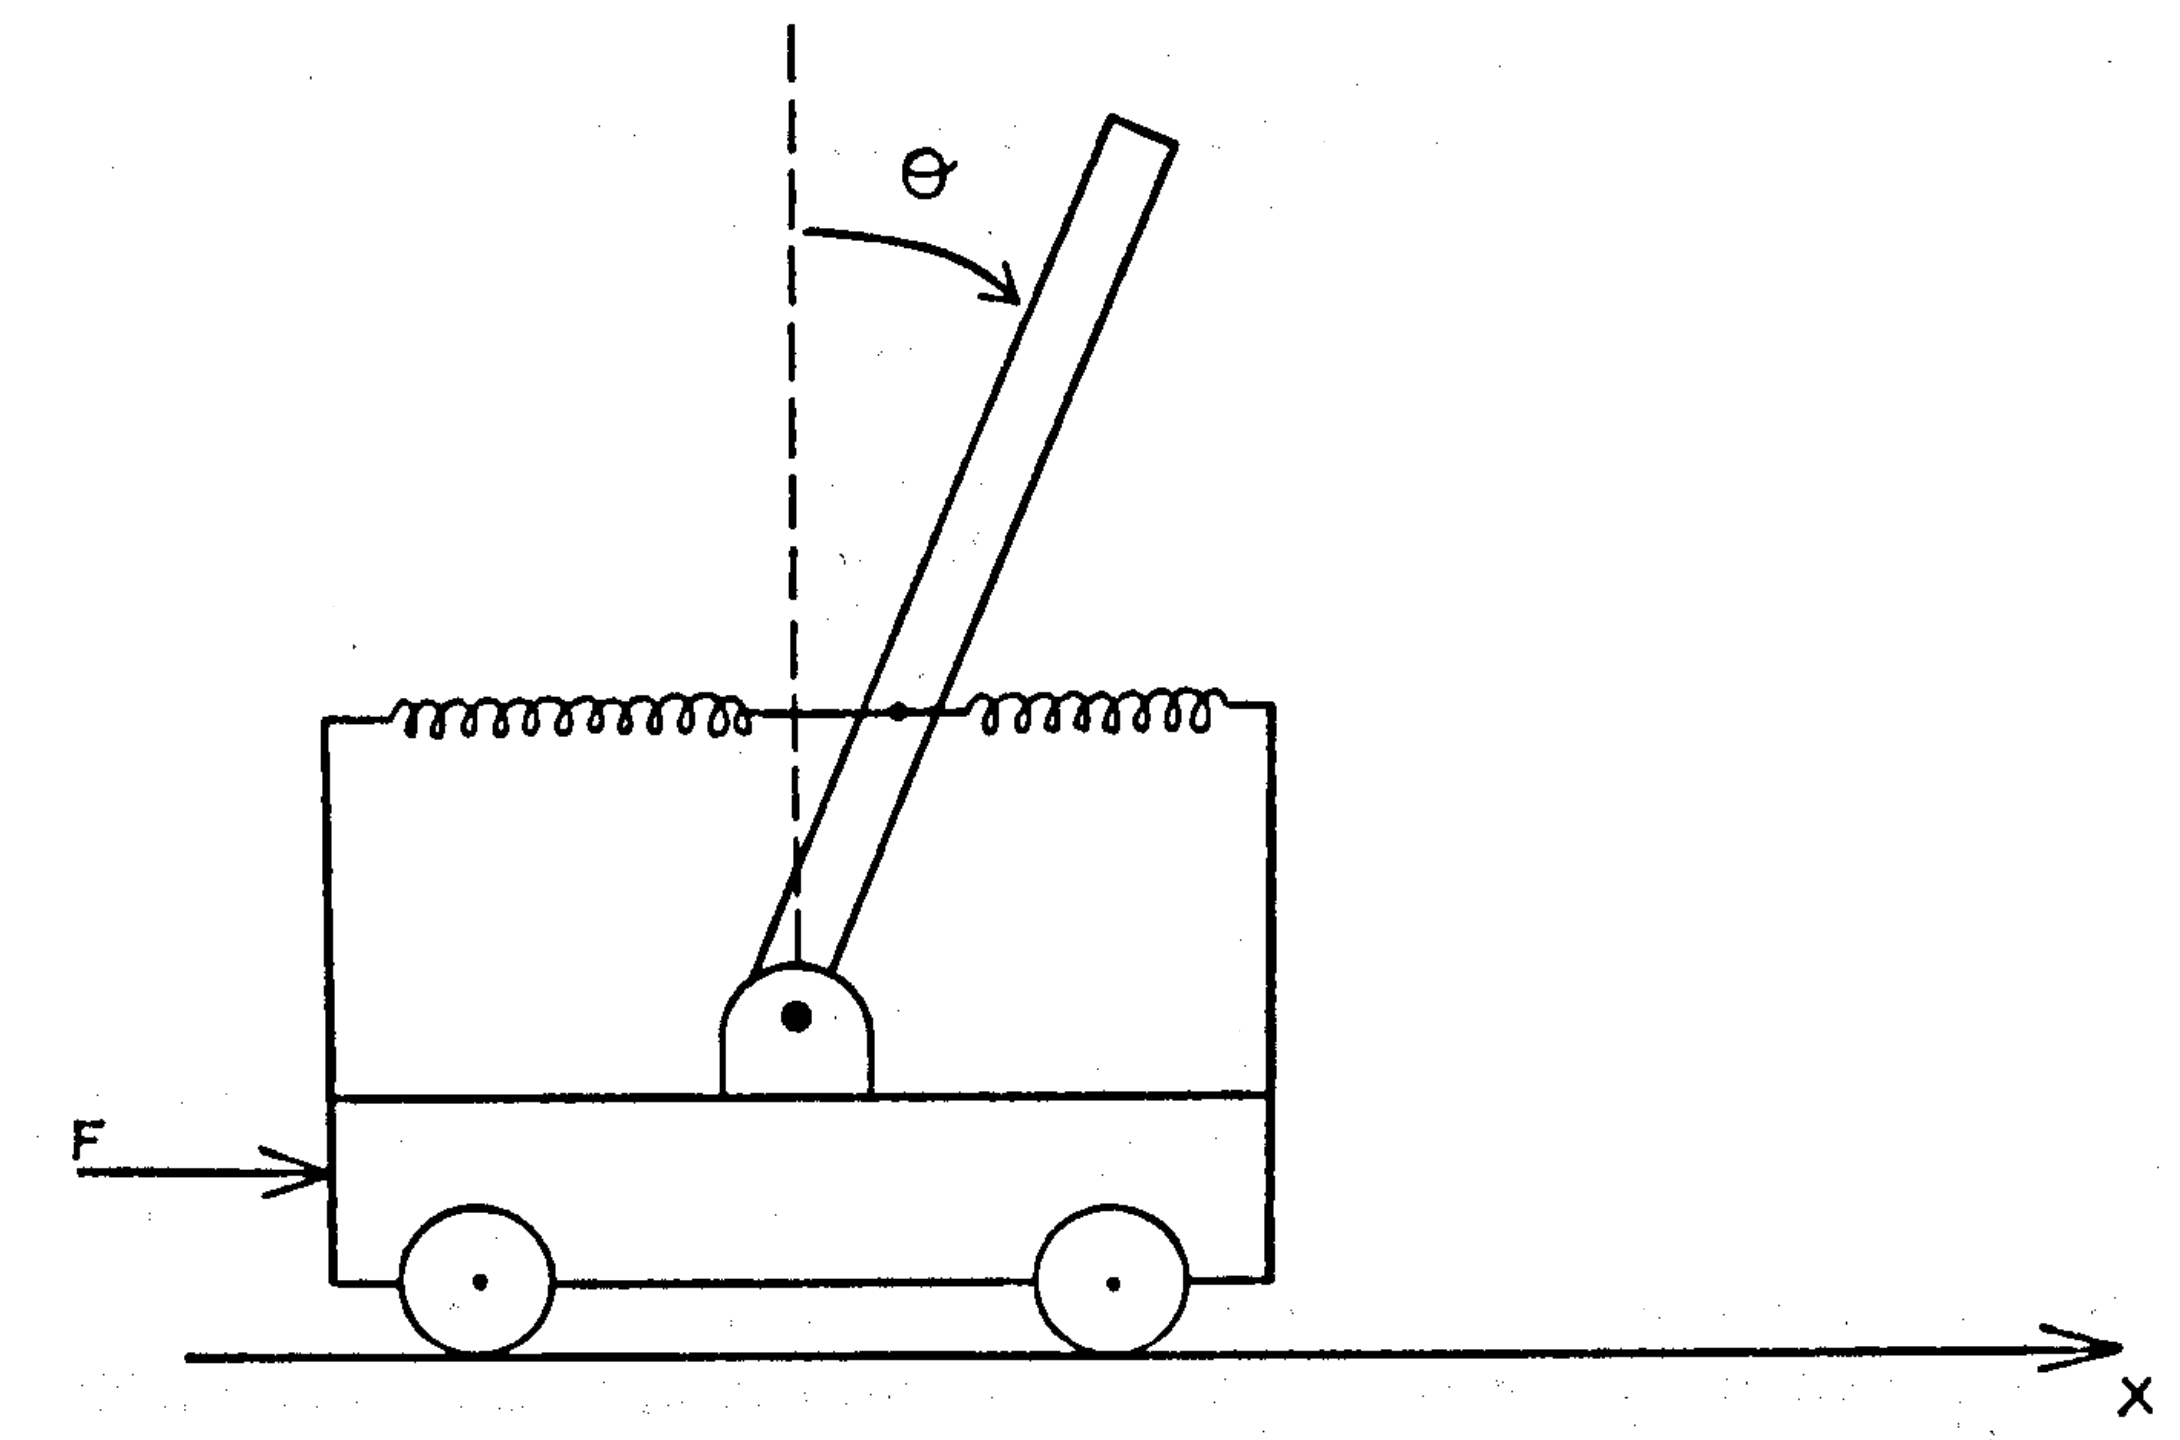
\includegraphics[width=1\linewidth]{portada.png}
    
\end{figure}

\thispagestyle{empty}
\newpage

\section{Detalles de implementación}

Motivados polo noso coñecemento teórico e a comprensión dos algoritmos non como secuencias de pasos que execútanse nun orden pero como principios teóricos que desembocan en implementacións; decidimos implementar a práctica dun xeito que reflictise as nosas creencias. Creiamos que, aínda que os algoritmos teñan propiedas moi distintas, son, polo menos dende algún punto de vista, moi similares tamén. Decidimos, entón, non implementar varias veces o mesmo código senón facelo o máis modular posibel. Foi tanta a sinxeleza que conseguimos, que aínda que o enunciado da práctica non pedise certas cousas (primeira visita ou non en MonteCarlo, inicialización informada, Sarsa Promedio ...), por completitude , foi moi doado conseguilo. Pódese ver abaixo un esquema do noso código. Donde unha clase abstracta \texttt{AlgoritmoAprendizaxeReforzo} define case todas as variables (arriba) e implementa case todos os métodos (abaixo) necesarios. Daquela \texttt{MonteCarlo} xa ten todo o que precisa para heredar e definir a súa clase. No caso dos algoritmos baseados en diferencias temporais, fixemos outra clase abstracta, que non implementando ningun algoritmo en concreto, só precisa tres liñas de Python por algoritmo particular que quera implementarse (e dicir: Sarsa, SarsaPromedio e Q-Aprendizaxe ocupan nove liñas en total). Isto foi posibel a partires da observación de que estes últimos só diferen no xeito de actualizar $Q(S,A)$.


\begin{figure}[h]
    \centering
    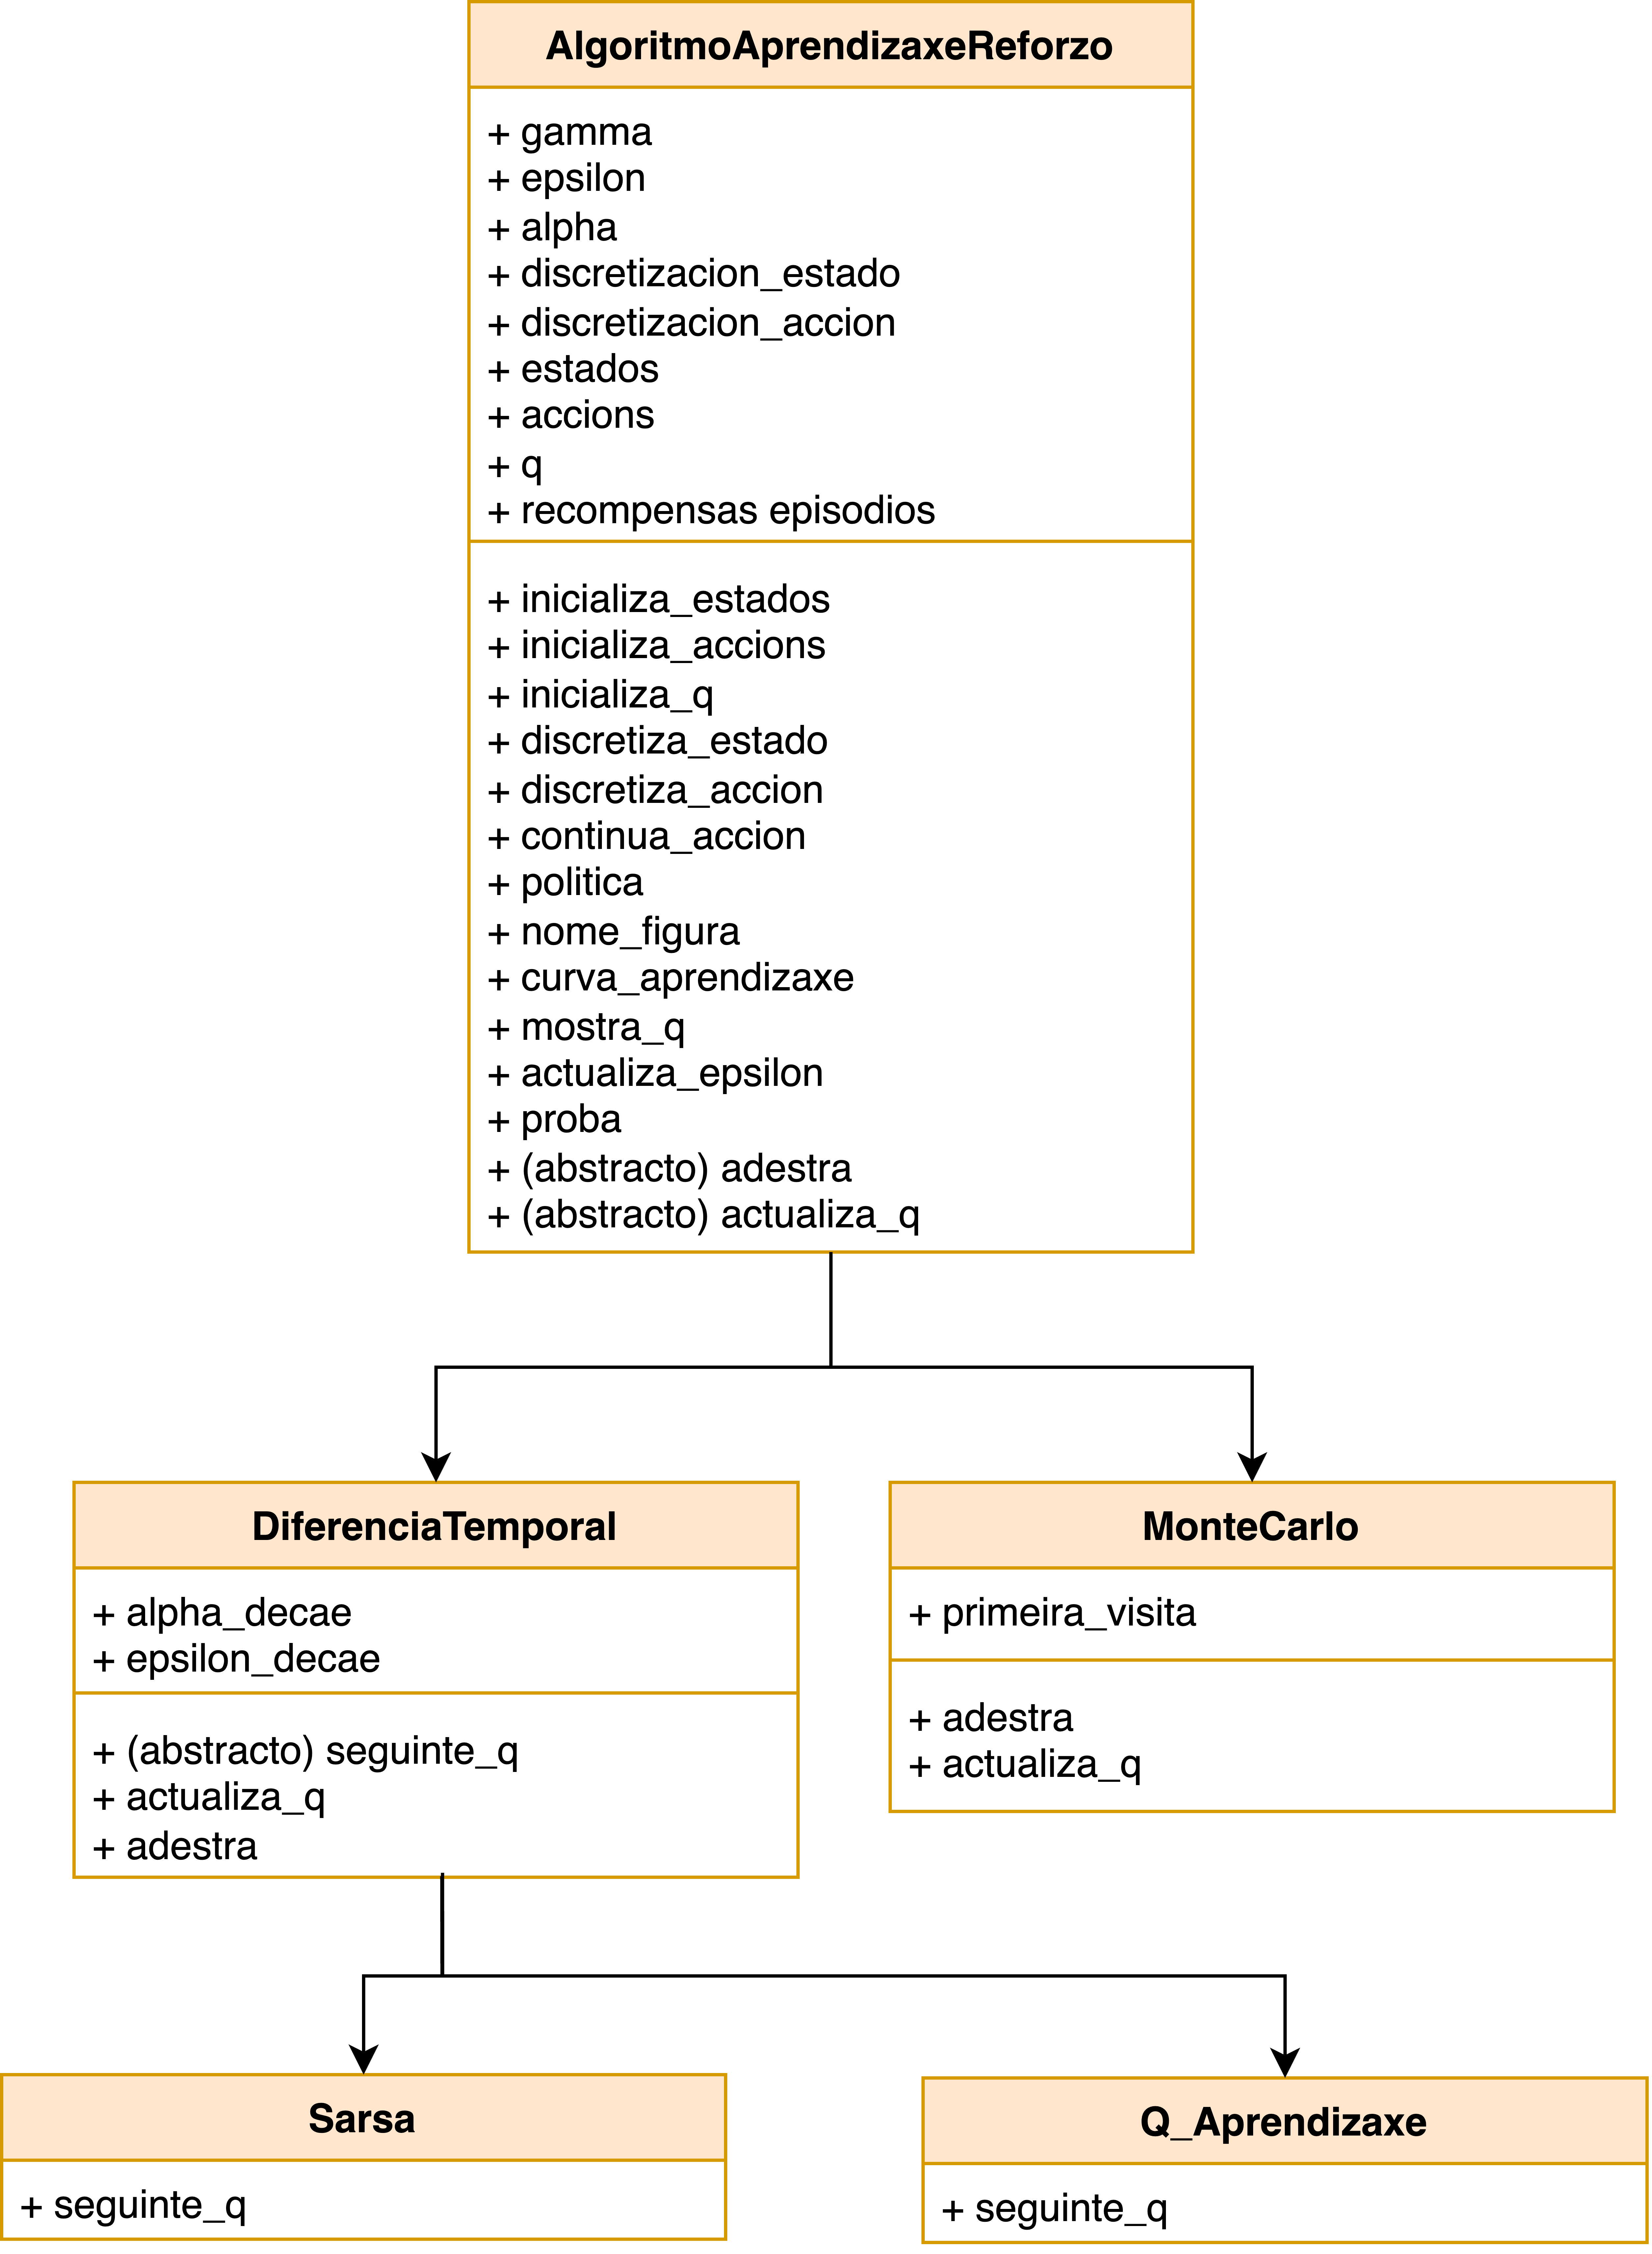
\includegraphics[width=0.7\linewidth]{herencia.drawio.png}
    
    \label{fig:enter-label}
\end{figure}

\section{Hiperparámetros}
Aínda que o problema a resolver é sixelo, a priori non sabemos (sobretodo sen experiencia) que hiperparámetros van resultar oportunos ou útiles, por tanto tentamos definir o maior número de hiperparámetros posibel; deste xeito, unha vez implementados só era cuestión de probar. Os hiperparámetros considerados e implementados ó largo do proceso foron:
\begin{itemize}
	\item \textbf{Número de iteracións.} Especialmente importante a súa combinación ca finura ou \emph{resolución} da discretización e cos decaementos doutros parámetros. Nunha das primeiras implementacións deixamos executando os tres algoritmos con 1M iteracións pero os resultados non pagan a pena (principalmente dado o alcance e obxectivo da práctica). Finalmente nos conformamos con 250K, que supón uns 6 minutos de adestramento, o cal é (pensamos) suficiente para obter resultados concluíntes. 
	\item \textbf{Número de pasos máximo.} Dende un primeiro momento deixamolo ó máximo porque en calqueira caso non eran episodios largos. 
	\item \textbf{Discretización do estado e acción.} A representación do estado non tivo en conta a natureza circular do problema. Deste xeito a nosa táboa Q é \emph{dispersa} (é dicir, moitas entradas permanecerán baleiras e inutilizadas). Nas probas que usamos máis finura de muestreo do espacio $(\text{cos}(\theta), \text{sin}(\theta),v) \subset \mathbb{R}^3$ (as presentadas aquí) contan de 30 valores posibles para magnitude, e como o estado é unha terna, máis a acción que é un único valor fan que a nosa táboa Q sexa un \emph{tensor} $(30\times 30 \times 30 \times 30)$. Inicialmente probamos (i) menor granularidade (ii) diferente finura para acción e estado. Os resultados suxiren que a configuración actual é millor. De todos xeitos o sentido común dí que máis finura sempre vai ofrecer polo menos resultados iguais ou millores. A nosa elección, por tanto, ten que ver co número de episodios elixido.
	\item \textbf{Parámetro $\gamma$.} En todo momento fixamos $\gamma = $ 0.99. Esta decisión respaldouse na unanimidade e consenso aparente cara este valor, despóis de buscar na Web. En calqueira caso con que sexa suficientemente alto é suficiente. Non ten, en cambio, porque ser igual a 1, de feito os episodios poderían ser infinitos.
	\item \textbf{Parámetro $\varepsilon$.} Cedo decatámosnos da importancia de este parámetro, motivo o cal decidimos implementar un decaemento (lineal) para que dentro dun aprendizaxe varie, acompañado de unha búsqueda \emph{manual}. En calqueira caso, o importante e que nos primeiros episodios sexa o suficientemente explorativo (alto $\varepsilon$) e nos finais que non tambalee e opte sempre polas mellores accións (baixo $\varepsilon$), esto pódese apreciar claramente co caso do SarsaPromedio. Aquí ó ter implementado o decaemento, empezar con un $\varepsilon$ alto significa ter a oportunidade de explorar máis opcións (potencialemte as óptimas). En ambas figuras, no final de todo $\varepsilon =$ 0.001.

		\begin{figure}[htbp]
    \centering
    \begin{minipage}{0.45\textwidth}
        \centering
        \includegraphics[width=\linewidth]{../cartafol/CA\_SarsaPromedio\_\_de\_30\_pert\_False\_da\_30\_g_0\%99\_e\_0\%5\_alpha\_0\%6.png}
\caption*{SarsaPromedio con $\varepsilon$ = 0.5}

    \end{minipage}
    \hfill
    \begin{minipage}{0.45\textwidth}
        \centering
        \includegraphics[width=\linewidth]{../cartafol/CA\_SarsaPromedio\_\_de\_30\_pert\_False\_da\_30\_g\_0\%99\_e\_0\%2\_alpha\_0\%2.png}
\caption*{SarsaPromedio con $\varepsilon$ = 0.2}

    \end{minipage}
\end{figure}

	\item \textbf{Parámetro $\alpha$.} Aínda que no Sutton e Barto \cite{Sutton1998}  propoñen unha versión do MonteCarlo que usa $\alpha$ dun xeito similar ós algoritmos de Diferencia Temporal:
			\[V(S_t)\leftarrow V(S_t)+\alpha[G_t -V(S_t)]\]

nós restrinximos o noso uso deste parámetro ós segundos. O que podemos dicir é moi parecido ó discurso de $\varepsilon$, implementar un decaemento lineal foi clave para poder actualizar sen problema ó principio, pero asegurar a converxencia ó final. A nosa búsqueda non foi necesariamente exhaustiva porque cedo atopamos valores que proporcionaben bos resultados ($\alpha =$ 0.6). Como particularidade, dicir que nun primeiro momento a implementación do decaemento era \emph{de potencia}, pero como foi suxerido en clase, finalmente nos quedamos coa lineal.

	\item \textbf{Parámetro booleano, inicialización informada.} Como o problema era tan sinxelo pensabamos que inicializando dun xeito naïve a táboa Q, teríamos vantaxe. Na nosa implementación penalizamos o movemento (queremeos que esté parado arriba), e beneficiamos as posición altas e os movementos que fosen en contra da velocidade do péndulo. En xeral non observamos grandes diferencias, ou ben porque non foi afortunada a nosa implementación ou ben porque efectivamente o problema era tan sinxelo que apenas viuse afectado.
	\item \textbf{Parámetro booleano, primeira visita.} Malia que os cadernos vistos na asignatura só presentaron a versión primeira visita do método MonteCarlo, sabemos pola lectura \cite{Sutton1998} que existe a outra posibilidade e pareceunos suficientemente tentadora como para querer implementala. Pódese ver o (pouco) efecto nas figuras de abaixo (os resultados en proba para estos experimentos pódense na Táboa \ref{tab:rl_algorithms}). Vese que con primeira visita, cando chega a 200K episodios xa ten a Recompensa total $G > 1000$ e non é certo no outro caso. Certamente a diferencia é minúscula (sabemos que asintóticamente non hai diferencia!) non obstante en adestramentos de moitos menos episodios sí pódese observarse algunha diferencia. En calqueira caso, ó poder dar a volta o pendulo, quizáis non sería esperable obter nunca moita diferencia, por esa propiedade cíclica.

		\begin{figure}[htbp]
    \centering
    \begin{minipage}{0.45\textwidth}
        \centering
	\includegraphics[width=\linewidth]{../cartafol/CA\_MonteCarlo\_\_de\_30\_pert\_False\_da\_30\_g\_0\%99\_e\_0\%5\_pv\_True.png}
\caption*{MonteCarlo con primeira visita}

    \end{minipage}
    \hfill
    \begin{minipage}{0.45\textwidth}
        \centering
	\includegraphics[width=\linewidth]{../cartafol/CA\_MonteCarlo\_\_de\_30\_pert\_False\_da\_30\_g\_0\%99\_e\_0\%5\_pv\_False.png}
\caption*{MonteCarlo sen primeira visita}

    \end{minipage}
\end{figure}


	\item \textbf{Parámetro booleano, decaementos.} Como adelantamos nas seccións de $\varepsilon$ e de $\alpha$, facer reducir os valores desos parametros co tempo ou non, sí entraña diferencia. Experimentalmente os resultados foron tan claros que xa cedo decidimos facer decaemento (en ambos parámetros).

\end{itemize}

Como definimos moitos hiperparámetros, naturalmente non podimos experimentar todas as combinacións, esto non foi un problema polos seguintes dous argumentos (i) o noso conocimiento teórico (aínda que por suposto, moi incompleto) peromitiunos dirixir a búsqueda e non probar cousas que ou ben non teñan sentido ou non iban mellorar os resultados (ii) o seren o problema tan sixelo, cedo acadamos con boas configuracións de hiperparámetros; poderiamos decir que, no espacio de hiperparámetros, para este problema, unha gran rexión conformaba eleccións aceptables de hiperparámetros. 

\newpage

\section{Mellor política determinista}

En canto a que algoritmo obtivo mellor política determinista, podemos dicir que Q Aprendizaxe, logo Sarsa, SarsaPromedio e por último MonteCarlo. Estos resultados obtivemolos do seguinte xeito: (i) entrenamos o necesario para xerar a Táboa \ref{tab:rl_algorithms} e de xeito automatico gardamos as respectivas táboas Q en arquivos \texttt{.npy} (ii) días despóis  cargamos estas táboas e fixemos un script que probase 1000 veces cada algoritmo e fixese a media. Para comprobar a vericidade dos nosos resultados (e se querese replicar o experimento), engadimos a forma de execución que empregamos: 


\begin{tcolorbox}[colback=black!5!white, colframe=black!75!white, title=Reproducir a táboa de debaixo]
\begin{lstlisting}[basicstyle=\ttfamily\small]
$ python proba.py | grep media
\end{lstlisting}
\end{tcolorbox}

Opcionalmente pódese cambiar as variables globales de devandito arquivo a (1, True) para ver cos ollos o comportamento do algoritmos.


\begin{table}[htbp]
\centering
\begin{tabular}{@{}ll@{}}
\toprule
Algoritmo     & Recompensa en proba \\ \midrule
Q Aprendizaxe & -149                                     \\ 
Sarsa         & -153                                     \\
SarsaPromedio & -251                                     \\
MonteCarlo    & -597                                     \\
\bottomrule
\end{tabular}
\end{table}

Os resultados son bastante esperables. Como Q Aprendizaxe aproxima $q_\star$ (a táboa Q de \emph{algunha} das políticas óptimas) en cada iteración en cal de $q_{\pi_{t}}$ (a táboa Q da política no instante $t$), e o adestramento foi con episodios suficientes, e natural que sexa o que o faga mellor. Sarsa, en cambio tambén o fixo moi ben porque como comentamos antes asíntoticamente son iguais. Sabemos que non é sempre Q Aprendizaxe mellor a Sarsa pero para este problema (que tiña no caso no-perturbado ningunha componente estócastica) sí é o caso.

Parecería unha sorpresa que SarsaPromedio dese peores resultados que os outros dous. Non o é. O algoritmo bó é SarsaEsperado, que fai a media dos $Q(S',a)$ ponderandoos con $\pi_t(a|S')$, nos por simplificación o fixemos ponderandoos con $\frac{1}{|\mathcal{A}(S')|}$. É dicir, non implementamos correctamente a expectación. Non podemos dicir que a nosa implementación valga para dicir nada concluente do comportamento de SarsaEsperado, máis podemos dicir que nos valeu para observar que, en efecto os detalles importan. Tanto así que (como pódese ver na Táboa \ref{tab:rl_algorithms}) baixo perturbacións ter en conta os $Q(S,A')$ para aquelas $A'$ non elixidas, empeora drásticamente os resultados; máis que nun entorno estable.

MonteCarlo, por outra banda queda nun segundo plano. Isto é porque MonteCarlo ten que esperar ó final de cada episodio para valorar e bondade das súas accións mentras que o resto de algoritmos o fan durante o mesmo episodio. Ademáis, MonteCarlo non sabe cales das accións que fixo nun mal episodio son malas nin cales das que fixo nun bo episodio son boas. É por isto que, para este problema, é esperable un peor rendimento por parte de MonteCarlo. 

\newpage

\section{Mellor algoritmo de control}


\epigraph{For the control problem (finding an optimal policy, DP, TD, and Monte Carlo methods all use some variation of generalized policy iteration (GPI). The differences in the methods are primarily differences in their approaches to the prediction problem.}

Ademáis da importancia que ten para un algoritmo comportarse ben unha vez está adestrado, é importante, sobretodo en Aprendizaxe por Reforzo, ofrecer bos comportamentos \emph{mentras} aprende. Baixo os nosos experimentos, os mellores algoritmos para esta cuestión son os mesmos e no mesmo orden que para o exercicio anterior.

Se ben o problema de \emph{mellor política determinista} redúcese a ver como o fan en proba (ou nos últimos episodios do adestramento se é que $\varepsilon$ decae ate moi baixo), en cambio este problema de \emph{mellor algoritmo de control} é relativo ó rendemento do algoritmo \emph{ó largo dos episodios.} Abaixo pódese ver unha comparativa cos mellores resultados por algoritmo da táboa \ref{tab:rl_algorithms}. Para mellor visulaización os resultados estan convolucionados cunha gausiana de $\sigma = \frac{\#episodios}{50}$. Independentemente do valor final obtido (o discutido no exercicio anterior) que verdaderamente é parecido o obtido nos tres métodos de Diferencia Temporal, pódese apreciar moi fácilmente as diferencias na velocidade de converxencia. Vemos que MonteCarlo necesita moitos episodios para comenzar a aprender significativamente e vemos que, dentro dos de Diferencia Temporal, Q Aprendizaxe e o que converxe máis rápido.

		\begin{figure}[htbp]
    \centering
    \begin{minipage}{0.45\textwidth}
        \centering
	\includegraphics[width=\linewidth]{../cartafol/CA\_MonteCarlo\_\_de\_30\_pert\_False\_da\_30\_g\_0\%99\_e\_0\%5\_pv\_True.png}
\caption*{MonteCarlo}

    \end{minipage}
    \hfill
    \begin{minipage}{0.45\textwidth}
        \centering
	\includegraphics[width=\linewidth]{../cartafol/CA\_Sarsa\_\_de\_30\_pert\_False\_da\_30\_g\_0\%99\_e\_0\%5\_alpha\_0\%6.png}
\caption*{Sarsa}

    \end{minipage}
    \hfill
    \begin{minipage}{0.45\textwidth}
        \centering
	\includegraphics[width=\linewidth]{../cartafol/CA\_SarsaPromedio\_\_de\_30\_pert\_False\_da\_30\_g\_0\%99\_e\_0\%5\_alpha\_0\%6.png}
\caption*{SarsaPromedio}

    \end{minipage}
    \hfill
    \begin{minipage}{0.45\textwidth}
        \centering
	\includegraphics[width=\linewidth]{../cartafol/CA\_Q\_Aprendizaxe\_\_de\_30\_pert\_False\_da\_30\_g\_0\%99\_e\_0\%2\_alpha\_0\%2.png}
\caption*{Q Aprendizaxe}

    \end{minipage}
\end{figure}

\newpage

Malia estos resultados semellar satisfactorios, ó principio extrañounos que Q Aprendizaxe fora o mellor polo seguinte comentario de \cite{Sutton1998}:

\begin{quote}
Although Q-learning actually learns the values of the optimal policy, its on-line performance is worse than that of Sarsa, which learns the roundabout policy. Of course, if $\varepsilon$ were gradually reduced, then both methods would asymptotically converge to the optimal policy.
\end{quote}

Entón, porque no noso experimento advertimos o contrario? Pensamos que débese a que o problema é tan sinxelo que ambos algoritmos só poden aprender o mesmo, é dicir, o óptimo. Entendemos que a circunstancia á que refirese o libro é dependente de entornos nos que existan solucións subóptimas ou triviais. Non é o caso co pendulo xa que non hai xeitos \emph{mellores} de manter o péndulo arriba. Por tanto ambos queren aprender $\pi_{\star}$ (\emph{algunha} política óptima), e Q Aprendizaxe ó facelo directamente é máis rápido.

\section{Perturbacións}

En canto ás perturbacións, planteamos os experimentos da seguinte forma: (i) adestrar o mesmo algoritmo con e sen perturbacións (como especificadas no enunciado da práctica) (ii) facer 5 episodios sen aprendizaxe, pero o que foi adestrado con perturbacións, tamén as terá en proba. Os resultados de este experimento, de novo, están na táboa \ref{tab:rl_algorithms}. En canto as curvas de aprendizaxe, son consistentemente (nos catro algoritmos) moi parecidas a versión con e sen perturbacións. Non pensamos que as perturbacións sexan meritorias de máis disimilitude polos seguintes argumentos:
\begin{itemize}
	\item Malia seren brutais no sentido de que a acción é extrema, ó ser con tan baixa probabilidad, non esperaríamos, de media, moita diferencia.
	\item En certa medida supón máis peso na parte de exploración e nese sentido as perturbacións son unha regularización.
	\item Aínda que as perturbacións están implementadas de xeito que enganan a percepción do axente (el pensa que fixo outra acción, e vai cambiar o $Q(S,a)$ de esa acción), só ocurre nun paso, no seguinte xa sabe onde está e (i) se aínda está a aprender, isto vale para facer máis exploración, (ii) se xa está aprendido, vai saber volver ó estado de inequilibro moi cedo. En calqueira caso, non hai moita disparidade. 

\end{itemize}

\section{Conclusións}

Os experimentos demostran que Q Aprendizaxe supera outros algoritmos tanto en calidade de políticas deterministas como en velocidade de converxencia, o que atribuese á súa aproximación directa da función acción-valor óptima. Sarsa e SarsaPromedio séguenlle de preto, mentres que Monte Carlo vai por detrás debido á súa natureza de aprendizaxe episódica. As perturbacións tiveron un impacto mínimo, o que suxire robustez nos deseños dos algoritmos. A implementación modular demostrou ser eficaz, permitindo extensións sen fisuras. 

Disfrutamos moito facendo a práctica porque o escenario tan académico non entorpeceu o noso acercamento a este novo paradigma de Aprendizaxe ate o momento descoñecido para nos. Esperamos, por outra banda, seguir aprendendo Aprendizaxe por Reforzo e mesmo usar as técnicas que xa coñecemos de Aprendizaxe si-no-semi-Supervisado. Para este problema seguramente fora máis axeitado unha representación non tabular do estado, porque baixo a nosa representación, todo o que aprenda dunha posición do pendulo dada con unha velocidade dada, non pode extrapolarlo a posicións e velocidades parecidas. 




\newpage

\section*{Anexo A: Experimentos}

Malia ter feito experimentos preliminares, os resultados que narranse na práctica, as figuras obtidas, e mesmo os arquivos \texttt{.npy} foron todos obtidos nunha única execución. 

\begin{tcolorbox}[colback=black!5!white, colframe=black!75!white, title=Reproducir a táboa de debaixo]
\begin{lstlisting}[basicstyle=\ttfamily\small]
$ chmod 777 ./script
$ ./script
$ python parser.py resultados.txt
\end{lstlisting}
\end{tcolorbox}


O \emph{script} tarda entre tres e catro horas en executarse e xenera as figuras e os arquivos \texttt{.npy}, tamén xera un arquivo cos resultados chamado \texttt{resultados.txt}, se parsease como indicado, obterase a táboa en \LaTeX do mesmo xeito que o temos feito nos.

\begin{table}[ht]
\centering
\begin{tabular}{|l|c|c|c|c|c|c|c|c|}
\hline
Algoritmo & $d_e$ & $d_a$ & Perturbación & $\gamma$ & $\alpha$ & $\epsilon$ & Primeira Visita & Recompensa en proba \\ \hline
MonteCarlo & 30 & 30 & False & 00.99 & - & 00.5 & False & -504.88 \\ \hline
MonteCarlo & 30 & 30 & False & 00.99 & - & 00.5 & True & -417.87 \\ \hline
Sarsa & 30 & 30 & False & 00.99 & 00.6 & 00.5 & - & -98.71 \\ \hline
Sarsa & 30 & 30 & False & 00.99 & 00.2 & 00.2 & - & -98.69 \\ \hline
SarsaPromedio & 30 & 30 & False & 00.99 & 00.6 & 00.5 & - & -121.81 \\ \hline
SarsaPromedio & 30 & 30 & False & 00.99 & 00.2 & 00.2 & - & -397.48 \\ \hline
Q Aprendizaxe & 30 & 30 & False & 00.99 & 00.6 & 00.5 & - & -132.64 \\ \hline
Q Aprendizaxe & 30 & 30 & False & 00.99 & 00.2 & 00.2 & - & -99.45 \\ \hline
MonteCarlo & 30 & 30 & True & 00.99 & - & 00.5 & True & -585.19 \\ \hline
Sarsa & 30 & 30 & True & 00.99 & 00.6 & 00.5 & - & -120.90 \\ \hline
SarsaPromedio & 30 & 30 & True & 00.99 & 00.6 & 00.5 & - & -361.70 \\ \hline
Q Aprendizaxe & 30 & 30 & True & 00.99 & 00.6 & 00.5 & - & -141.05 \\ \hline
\end{tabular}
\caption{Comparación de hiperparámetros e algoritmos.}
\label{tab:rl_algorithms}
\end{table}

A columna Recompensa en Proba é a media de 5 episodios sen aprendizaxe baixo as mesmas condicións de perturbación ou non que o adestramento. 

\newpage


\bibliographystyle{plain}  % or another style like "ieeetr", "acm", "alpha", etc.
\bibliography{articulos_mencionados}  % 'references' is the name of your .bib file (without the extension)



\end{document}

